\documentclass[12pt, t, xcolor=dvipsnames]{beamer}
\usepackage{xspace}
\usepackage{appendixnumberbeamer}
\usepackage{xcolor}
\usepackage{minted}
\usepackage[scale=2]{ccicons}
\usepackage{booktabs}
\usepackage{graphicx}
% \usepackage[absolute,overlay]{textpos}
\usepackage{pgfplots}
\usepackage{hyperref}


\useoutertheme{metropolis}
\useinnertheme{metropolis}
\usefonttheme{metropolis}
\usecolortheme{metropolis}

\pgfplotsset{compat=1.14}

\setbeamercolor{normal text}{fg=black!95, bg=white}
%\setbeamersize{text margin left=6mm, text margin right=6mm} 
\setlength{\leftmargini}{0pt}

\usemintedstyle{borland}

\graphicspath{ {figures/} }

\setbeamercolor{framesource}{fg=gray}
\setbeamerfont{framesource}{size=\tiny}

\makeatletter
\renewcommand{\footnoterule}{}
\define@key{beamerfootnote}{nonumber}[true]{\edef\beamer@footarg{0}\def\@makefnmark{}}% have to set a number in \beamer@footarg, then it won't be automatically generated one. setting \@makefnmark to be empty means the number isn't printed. but only use this in a group else it affects following footnotes!
% instead of 'nonumber', could just use 0 as an optional argument to \footnote, but OP reports that keyval complains about this in some situations
% http://tex.stackexchange.com/questions/89539
\newcommand{\source}[1]{{\footnote[nonumber]{%
    \begin{beamercolorbox}[right,wd=\dimexpr\hsize-1.8em\relax]{framesource}
      \usebeamerfont{framesource}\usebeamercolor[fg]{framesource} Source: {#1}
    \end{beamercolorbox}}}}
\setlength{\footnotesep}{0cm}%\footnotesep is the space between footnotes (generated with a \rule)
\makeatother

% inspired by [beamer: footnote text collides with navigation symbols](http://tex.stackexchange.com/a/5855)
\addtobeamertemplate{sidebar right}{\setbeamertemplate{navigation symbols}{}}{}
\addtobeamertemplate{footline}{\hfill\usebeamertemplate***{navigation symbols}%
    \hspace*{0.1cm}\par\vskip 2pt}{}

% \setbeamercolor{framesource}{fg=gray}
% \setbeamerfont{framesource}{size=\tiny}
% 
% \newcommand{\source}[1]{\begin{textblock*}{4cm}(8.7cm,8.6cm)
%     \begin{beamercolorbox}[ht=0cm,right]{framesource}
%         \usebeamerfont{framesource}\usebeamercolor[fg]{framesource} Source: {#1}
%     \end{beamercolorbox}
% \end{textblock*}}

\tikzset{
  every overlay node/.style={
    draw=black,fill=white,rounded corners,anchor=north west,
  },
}

\def\tikzoverlay{%
   \tikz[baseline,overlay]\node[every overlay node]
}%

\definecolor{codegray}{gray}{0.95}
\newcommand{\code}[1]{\colorbox{codegray}{\textcolor{black!95}{\texttt{#1}}}}
%\newcommand{\code}[1]{\texttt{#1}}}

\newminted{R}{fontsize=\scriptsize, 
              frame=lines,
              bgcolor=codegray,
              framesep=1mm}

\newcommand {\framedgraphic}[2] {
    \begin{frame}{#1}
        \begin{center}
            \includegraphics[width=\textwidth,height=0.8\textheight,keepaspectratio]{#2}
        \end{center}
    \end{frame}
}

\pgfmathdeclarefunction{gauss}{3}{%
  \pgfmathparse{1/(#3*sqrt(2*pi))*exp(-((#1-#2)^2)/(2*#3^2))}%
}

\title{Week 2 Lab}
% \subtitle{}
\date{\today}
\author{Yuanchao Zhang}
% \institute{}
% \titlegraphic{\hfill\includegraphics[height=1.5cm]{logo.pdf}}
\renewcommand\appendixname{Appendix}

\begin{document}

\maketitle

\begin{frame}{Plan for today}
  \setbeamertemplate{section in toc}[sections numbered]
  \tableofcontents[hideallsubsections]
\end{frame}


\section{Changes of lab session administration}

\begin{frame}{Changes of lab session administration}
  \begin{itemize}
    \item Lab handout:
    \begin{itemize}
       \item Merged to homework assignment.
       \item Written mostly by instructors.
     \end{itemize}
    \item Optional sections of lab handout:
    \begin{itemize}
       \item Separated from the handout \& homework assignment.
       \item Will show up in the "\alert{Pages}" section of Canvas.
     \end{itemize}
  \end{itemize}
\end{frame}

\section{Recap}

\begin{frame}{Recap}
  \begin{itemize}
    \item R environment
    \begin{itemize}
      \item Associated with each R interpreter session
    \end{itemize}
    
    \item R current working directory
    \begin{itemize}
      \item Do \alert{NOT} change during analysis
    \end{itemize}
    
    \item Path
    \begin{itemize}
      \item Absolute path
      \item Relative path
      \item Path delimiter:
      \begin{itemize}
        \item \code{\textbackslash} in Windows
        \item \code{/} in Linux and MacOS
        \item \code{/} in R works for Windows, Linux, and MacOS
      \end{itemize}

    \end{itemize}
  \end{itemize}
\end{frame}

\begin{frame}{Recap}
  \begin{itemize}
    \item Tutorial of R data analysis
    \begin{itemize}
      \item Input: 
      \begin{itemize}
        \item \code{read.csv()}
      \end{itemize}
      
      \item Analyze: 
      \begin{itemize}
        \item Plotting: \code{ggplot2}
        \item Data manipulation: indexing, \code{subset()}, and \code{dplyr}
        \item Statistical testing: \code{t.test()}
      \end{itemize}
      
      \item Output: \code{write.csv()} and \code{pdf()}
    \end{itemize}

  \end{itemize}

\end{frame}


\section{Install packages}

\begin{frame}[fragile]{Install packages}
\begin{Rcode}
# For normality test
install.packages('nortest')

# For power analysis of one sample proportion test
install.packages('pwr')

# You do not need to run this if you already
# installed `ggplot2'
install.packages('ggplot2')
\end{Rcode}
\end{frame}

\section{The normal distribution}

\subsection{Mathematical properties}

\begin{frame}{The normal distribution}

When a random variable $X$ is dristributed normally with mean $\mu$ and variance $\sigma^2$, we write:
\[ X \sim \mathcal{N}(\mu,\,\sigma^{2}) \]

Probability density distribution (PDF) of the normal distribution:

\[ f(x|\mu, \sigma^2) = \frac{1}{\sqrt{2\pi\sigma^2}} e ^ { -\frac{ (x-\mu)^2 }{2\sigma^2} } \]

\source{\href{https://en.wikipedia.org/wiki/Normal_distribution}{Normal Distribution at en.wikipedia.org}}

\end{frame}


\begin{frame}{PDF of the normal distribution}
\[ f(x|\mu, \sigma^2) = \frac{1}{\sqrt{2\pi\sigma^2}} e ^ { -\frac{ (x-\mu)^2 }{2\sigma^2} } \]

\begin{tikzpicture}
\begin{axis}[
  no markers, 
  domain=0:6, 
  samples=100,
  ymin=0,
  axis lines*=left, 
  xlabel=$x$,
  ylabel={$f(x | \mu, \sigma^2)$},
  every axis y label/.style={at=(current axis.above origin),anchor=south},
  every axis x label/.style={at=(current axis.right of origin),anchor=west},
  height=5cm, 
  width=12cm,
  xtick=\empty, 
  ytick=\empty,
  enlargelimits=false, 
  clip=false, 
  axis on top,
  grid = major,
  ]

 \addplot [very thick,cyan!50!black] {gauss(x, 3, 1)};

\pgfmathsetmacro\valueA{gauss(1,3,1)}
\pgfmathsetmacro\valueB{gauss(2,3,1)}
\pgfmathsetmacro\valueC{gauss(3,3,1)}
\draw [gray] (axis cs:1,0) -- (axis cs:1,\valueA)
    (axis cs:5,0) -- (axis cs:5,\valueA);
\draw [gray] (axis cs:2,0) -- (axis cs:2,\valueB)
    (axis cs:4,0) -- (axis cs:4,\valueB);
\draw [gray] (axis cs:3,0) -- (axis cs:3,\valueC);
\draw [yshift=1.4cm, latex-latex](axis cs:2, 0) -- node [fill=white] {$0.683$} (axis cs:4, 0);
\draw [yshift=0.4cm, latex-latex](axis cs:1, 0) -- node [fill=white] {$0.954$} (axis cs:5, 0);

\node[below] at (axis cs:1, 0)  {$\mu - 2\sigma$}; 
\node[below] at (axis cs:2, 0)  {$\mu - \sigma$}; 
\node[below] at (axis cs:3, 0)  {$\mu$}; 
\end{axis}
\end{tikzpicture}

\source{\href{https://tex.stackexchange.com/questions/100022/plotting-normal-distribution-in-pgfplots/100030\#100030}{Jake at TeXExchange}}

\end{frame}

\begin{frame}{The normal distribution}
\begin{tikzpicture}
\begin{axis}[
  no markers, 
  domain=0:6, 
  samples=100,
  ymin=0,
  axis lines*=left, 
  xlabel=$x$,
  ylabel={$f(x | \mu, \sigma^2)$},
  every axis y label/.style={at=(current axis.above origin),anchor=south},
  every axis x label/.style={at=(current axis.right of origin),anchor=west},
  height=3cm, 
  width=10cm,
  xtick=\empty, 
  ytick=\empty,
  enlargelimits=false, 
  clip=false, 
  axis on top,
  grid = major,
  ]

 \addplot [very thick,cyan!50!black] {gauss(x, 3, 1)};

\pgfmathsetmacro\valueA{gauss(1,3,1)}
\pgfmathsetmacro\valueB{gauss(2,3,1)}
\pgfmathsetmacro\valueC{gauss(3,3,1)}
\draw [gray] (axis cs:1,0) -- (axis cs:1,\valueA)
    (axis cs:5,0) -- (axis cs:5,\valueA);
\draw [gray] (axis cs:2,0) -- (axis cs:2,\valueB)
    (axis cs:4,0) -- (axis cs:4,\valueB);
\draw [gray] (axis cs:3,0) -- (axis cs:3,\valueC);

\node[below] at (axis cs:1, 0)  {$\mu - 2\sigma$}; 
\node[below] at (axis cs:2, 0)  {$\mu - \sigma$}; 
\node[below] at (axis cs:3, 0)  {$\mu$}; 
\end{axis}
\end{tikzpicture}

    \begin{itemize}
    \item Single Peaked
    \item Symmetric
    \item $E[x]=\mu$
    \item $Var[x]=\sigma^{2}$
    \item $SD[x]=\sigma$
    \end{itemize}

    \source{Paul E. Johnson. CLT. 2011}
\end{frame}

\subsection{Generate normal random numbers with \texttt{rnorm}}

\begin{frame}[fragile]{Generate normal random numbers with \code{rnorm}}
\begin{Rcode}
opar <- par(no.readonly = TRUE)
par(mfrow=c(2, 2)) 
normdata <- rnorm(10, mean=0, sd=1) 
hist(normdata)
hist(normdata)
par(opar)
\end{Rcode}

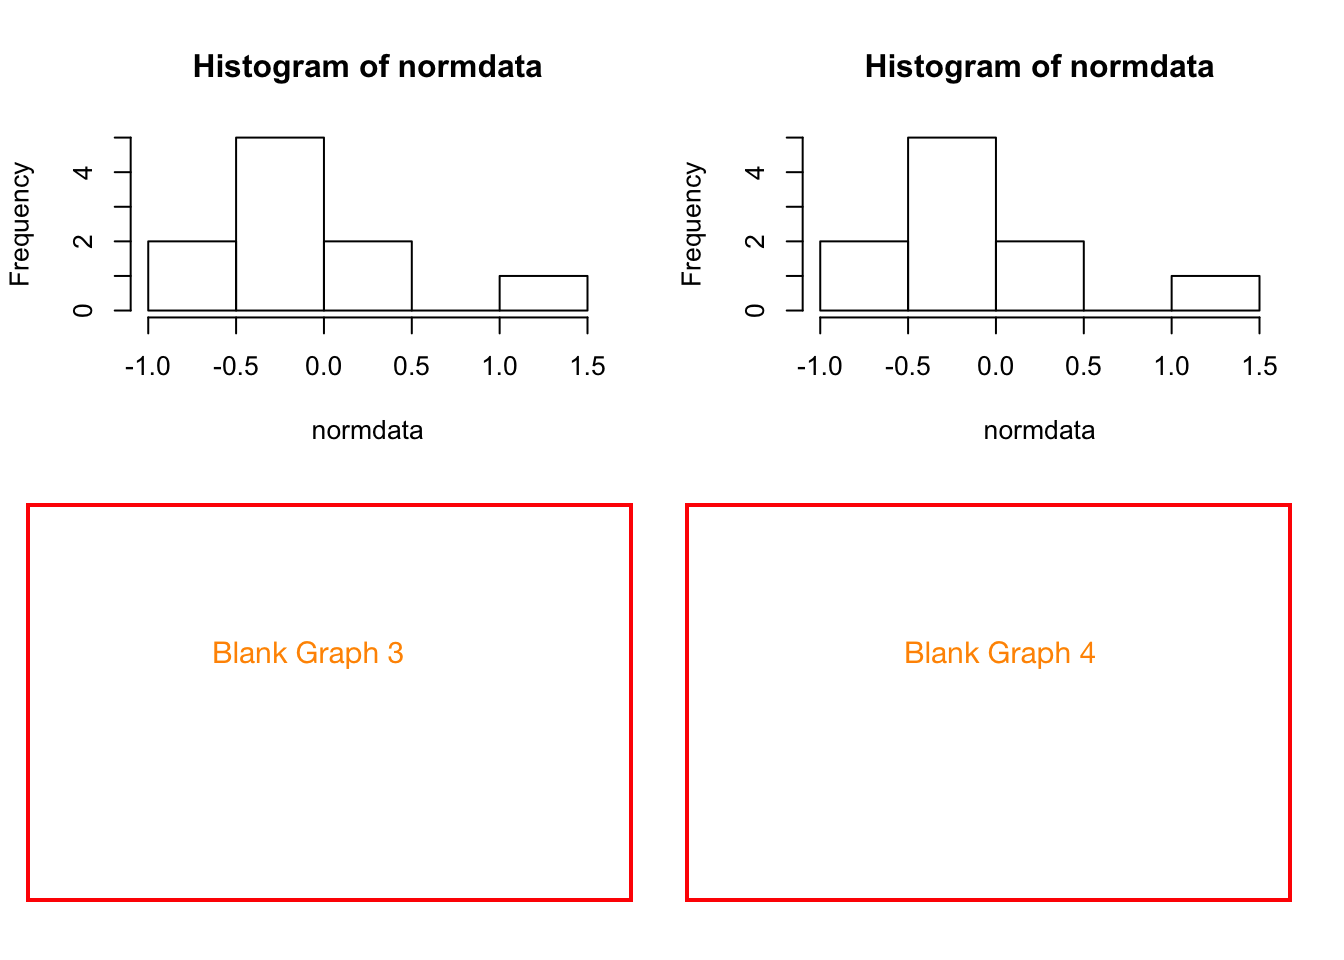
\includegraphics[width=\linewidth, height=0.5\textheight, keepaspectratio]{his22}
\end{frame}

\framedgraphic{\code{par(mfrow=c(2, 2))}}{his22}

\begin{frame}[fragile]{\code{par(opar)}}
\begin{Rcode}
# Plotting parameters have been set to old ones
# in `opar'
hist(normdata)
\end{Rcode}
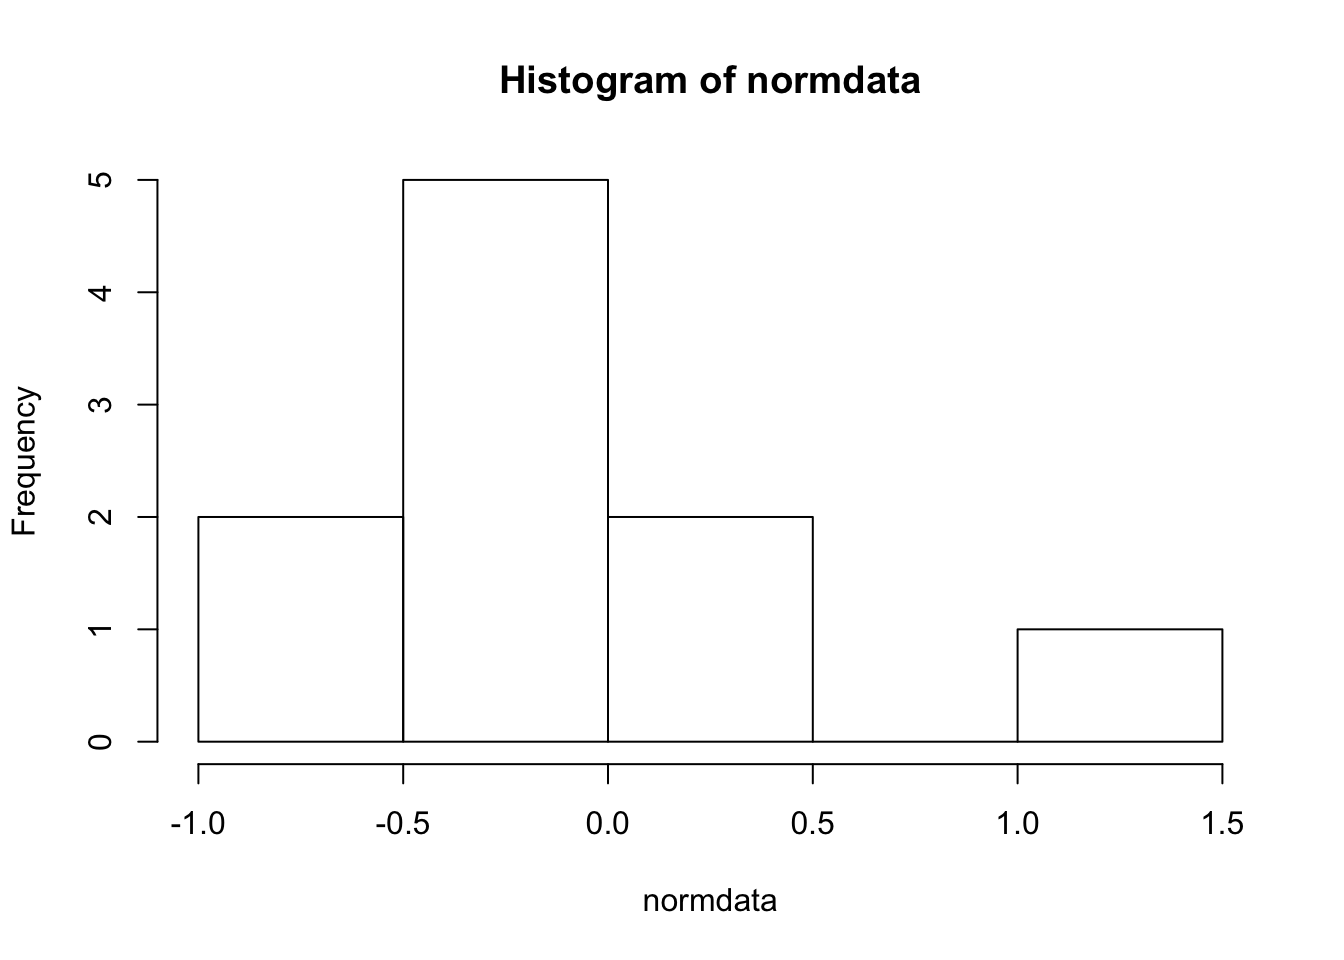
\includegraphics[height=0.6\textheight, keepaspectratio]{his11}
\end{frame}


\begin{frame}[fragile]{Generate normal random numbers with \code{rnorm}}
\begin{Rcode}
normdata <- rnorm(10, mean=0, sd=1) 
mean(normdata)
## [1] -0.1397156
sd(normdata)
## [1] 0.5693181
\end{Rcode}
\end{frame}

\begin{frame}[fragile]{Generate 1 million normal random numbers}
\begin{Rcode}
normdata <- rnorm(1000000, mean=0, sd=1) 
mean(normdata)
## [1] -9.904492e-05
sd(normdata)
## [1] 1.000252
hist(normdata)
\end{Rcode}
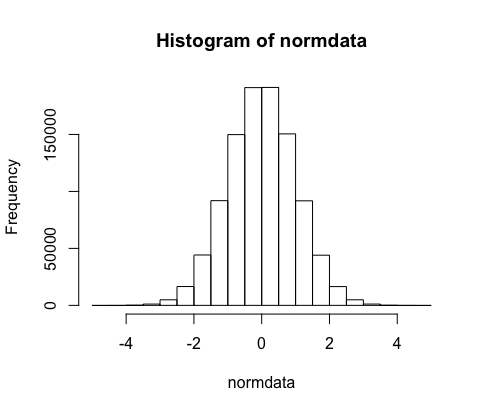
\includegraphics[height=0.5\textheight, keepaspectratio]{rnorm1m}
\end{frame}


\begin{frame}[fragile]{Calculate probability density of normal distribution with \code{dnorm}}
\begin{Rcode}
z_score_range <- seq(-4, 4, by = 0.2)
den_zscores <- dnorm(z_score_range)
plot(den_zscores, type = "l", 
     main = "PDF on the Standard Normal Distribution", 
     xlab = "Z-score", ylab = "Density", xaxt = "n")

den_zscore_sigmas <- c(dnorm(4), dnorm(3), dnorm(2), 
                       dnorm(1), dnorm(0), dnorm(1), 
                       dnorm(2), dnorm(3), dnorm(4))

den_score_labels <- c(-4, -3, -2, -1, 0, 1, 2, 3, 4)
axis(1, at = which(den_zscores %in% den_zscore_sigmas), 
     labels = den_score_labels)
\end{Rcode}
\end{frame}

\begin{frame}{Calculate probability density of normal distribution with \code{dnorm}}
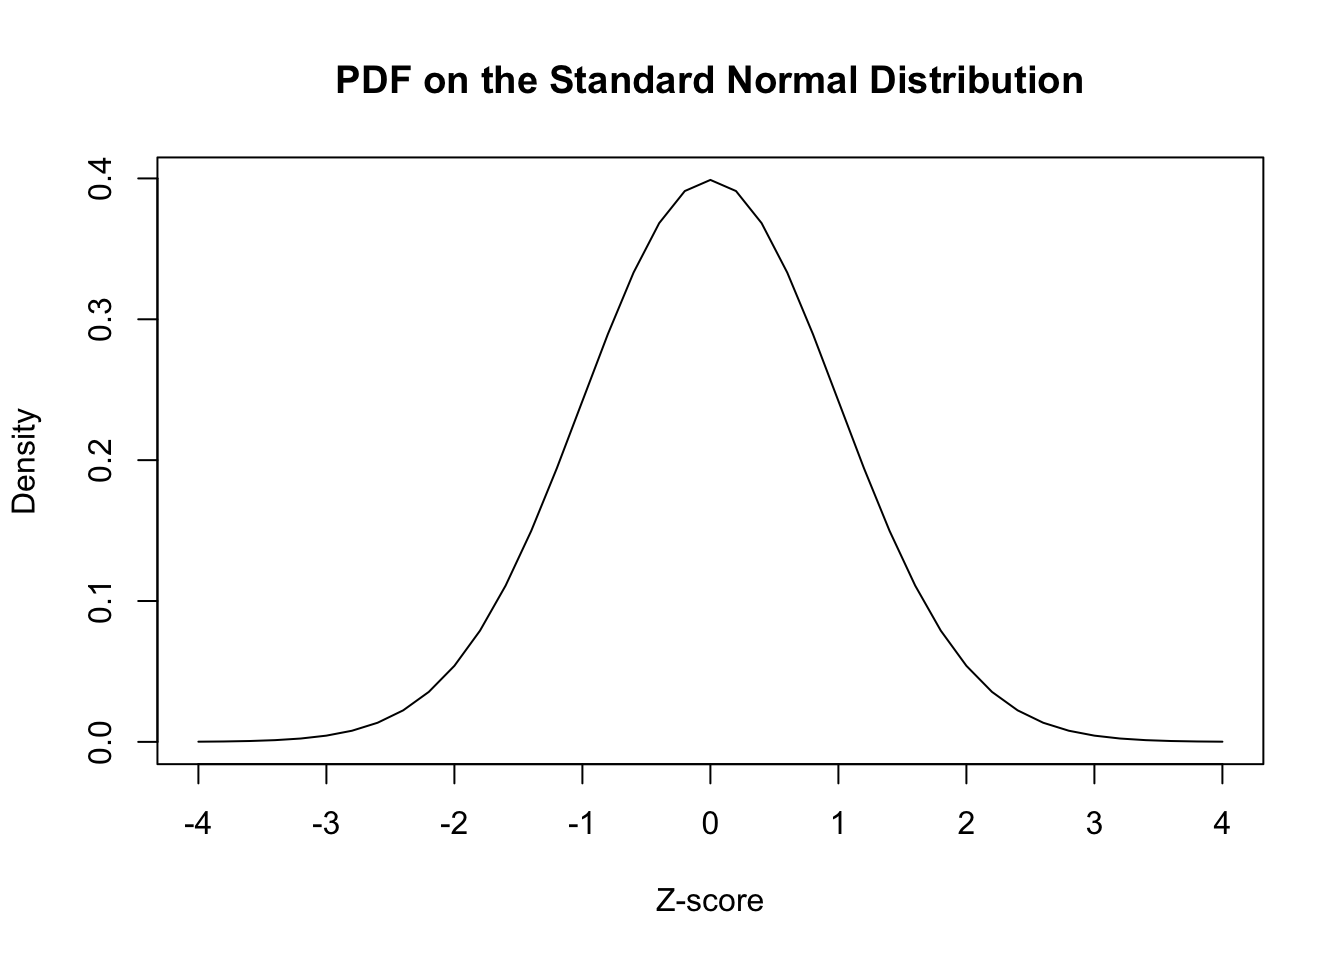
\includegraphics[width=\textwidth, height=\textheight, keepaspectratio]{dnorm}
\end{frame}


\begin{frame}[fragile]{Calculate cumulative probability of normal distribution with \code{pnorm}}
\begin{Rcode}
pnorm_scores <- pnorm(z_score_range)
plot(pnorm_scores, type = "l", 
     main = "CDF of the Normal Distribution", 
     xlab = "quantile", ylab = "density", xaxt = "n")

pnorm_values <- c(pnorm(-4), pnorm(-3), pnorm(-2), 
                  pnorm(-1), pnorm(0), pnorm(1), 
                  pnorm(2), pnorm(3), pnorm(4))

axis(1, at = which(pnorm_scores %in% pnorm_values), 
     labels = round(pnorm_values, 4), las = 3)
\end{Rcode}
\end{frame}

\begin{frame}{Calculate probability density of normal distribution with \code{dnorm}}
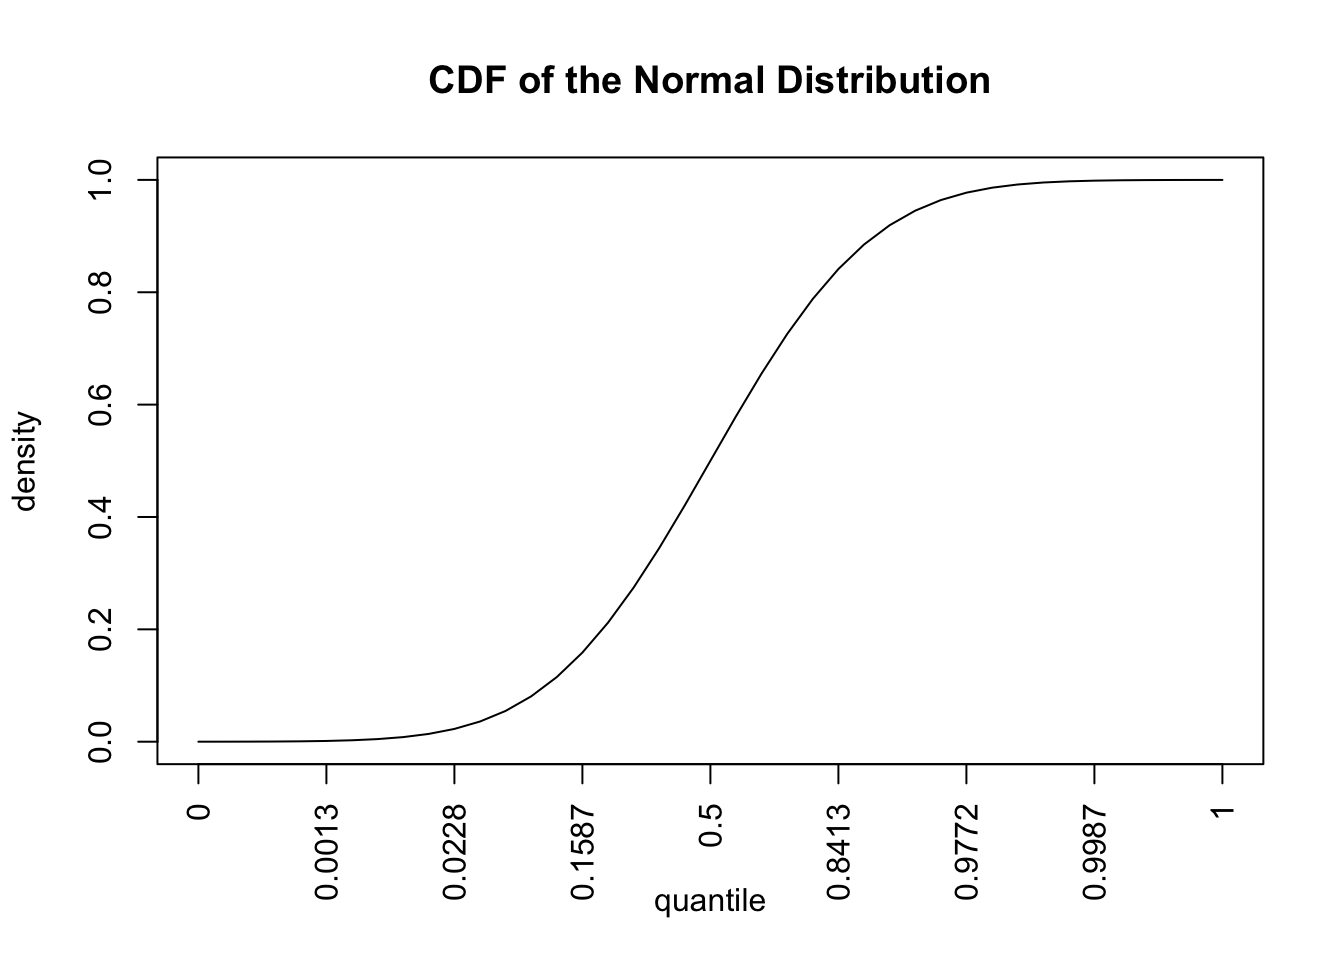
\includegraphics[width=\textwidth, height=\textheight, keepaspectratio]{pnorm}
\end{frame}

\begin{frame}[fragile]{Calculate quantiles of normal distribution with \code{qnorm}}
\begin{Rcode}
qnorm(0.99)
## [1] 2.326348

qnorm(0.9999)
## [1] 3.719016

pnorm(qnorm(0.9999))
## [1] 0.9999

# lower.tale: if TRUE (default), probabilities are P[X ≤ x] 
# otherwise, P[X > x].
qnorm(0.9999, lower.tail = FALSE)
## [1] -3.719016

qnorm(1e-04)
## [1] -3.719016

pnorm(qnorm(0.9999, lower.tail = FALSE))
## [1] 1e-04
\end{Rcode}
\end{frame}




\subsection{Central limit theorem}

\begin{frame}{Central limit theorem}

\begin{Theorem}

Let ${X_1, X_2, ..., X_n}$ be a sequence of identically distributed ($i.i.d.$) random variables with mean $E \left[{X_i}\right] = \mu$ and finite variance $Var \left({X_i}\right) = \sigma^2$ . 
Define $\displaystyle S_n = \frac{1}{n} \sum_i X_i$ . Then, as $n \to \infty$, $\displaystyle S_n \xrightarrow {\mathcal{D}} \mathcal{N} \left({\mu,\sigma^2/n}\right).$

\end{Theorem}

\vspace{3mm}

Central limit theorem is difficult to prove algebraically, but it is
quite easy to demonstrate with simulation. 

\source{Central Limit Theorem at en.wikipedia.org}

\end{frame}


\begin{frame}{Demonstrate central limit theorem with simulation}
\begin{Theorem}

Let ${X_1, X_2, ..., X_n}$ be a sequence of $i.i.d.$ random variables with mean $E \left[{X_i}\right] = \mu$ and finite variance $Var \left({X_i}\right) = \sigma^2$ . 
Define $\displaystyle S_n = \frac{1}{n} \sum_i X_i$ . Then, as $n \to \infty$, $\displaystyle S_n \xrightarrow {\mathcal{D}} \mathcal{N} \left({\mu,\sigma^2/n}\right).$

\end{Theorem}

\begin{itemize}
  \item Simulation procedure:
  \begin{enumerate}
    \item Let ${X_1, X_2, ..., X_n}$ be a sequence of i.i.d. uniformly distributed random variables.
    \item Calculate sample everage $S_n$. 
    \item Repeat $m$ times. 
    \item Plot the empirical PDF of $S_n$ and normal PDF stated by the theorem. 
  \end{enumerate}
\end{itemize}

\end{frame}

\begin{frame}[fragile]{Demonstrate central limit theorem with simulation}

\begin{Rcode}
# Let X1, X2, ..., X10 be a sequence of i.i.d. 
# random variables uniformly distributed 
# from 0 to 1.
runif(n = 10, min = 0, max = 1)
##  [1]  0.89804708 0.85956656 0.63841285 
##  [4]  0.59958342 0.68575572 0.28295208
##  [7]  0.42904749 0.15577247 0.26559273
##  [10] 0.01854827
\end{Rcode}

\end{frame}


\begin{frame}[fragile]{Demonstrate central limit theorem with simulation}

\begin{minted}[fontsize=\scriptsize,
               frame=lines,
               bgcolor=codegray,
               framesep=1mm]{R}
number_of_samples <- 5000
size_of_each_sample <- 5000
unif_min <- 0
unif_max <- 100

unif_mean <- (unif_max - unif_min) / 2
unif_sd <- (((unif_max - unif_min) ^ 2) / 12) ^ 0.5

sample_average_vector <- replicate(number_of_samples, {
  mean(runif(n = size_of_each_sample, 
             min = unif_min, 
             max = unif_max))
})
\end{minted}
\end{frame}

\begin{frame}[fragile]{Demonstrate central limit theorem with simulation}

\begin{minted}[fontsize=\scriptsize,
               frame=lines,
               bgcolor=codegray,
               framesep=1mm]{R}
clt_norm_mean <- unif_mean
clt_norm_sd <- unif_sd / (size_of_each_sample ^ 0.5)

ggplot(data = data.frame(x = sample_average_vector), 
       mapping = aes(x = x)) +
  geom_histogram(mapping = aes(y = ..density..), 
                 alpha = 0.4) +
  geom_density(mapping = aes(color = 'Sample Ave. Dens.')) +
  stat_function(fun = dnorm, 
                args = list(mean=clt_norm_mean, 
                            sd=clt_norm_sd), 
                aes(colour = 'CLT Norm. Dens.')) + 
  labs(x = 'Sample Average', y = 'Density') + 
  ggtitle("Central Limit Theorem Simulation")
\end{minted}

\end{frame}


\begin{frame}{Demonstrate central limit theorem with simulation}
  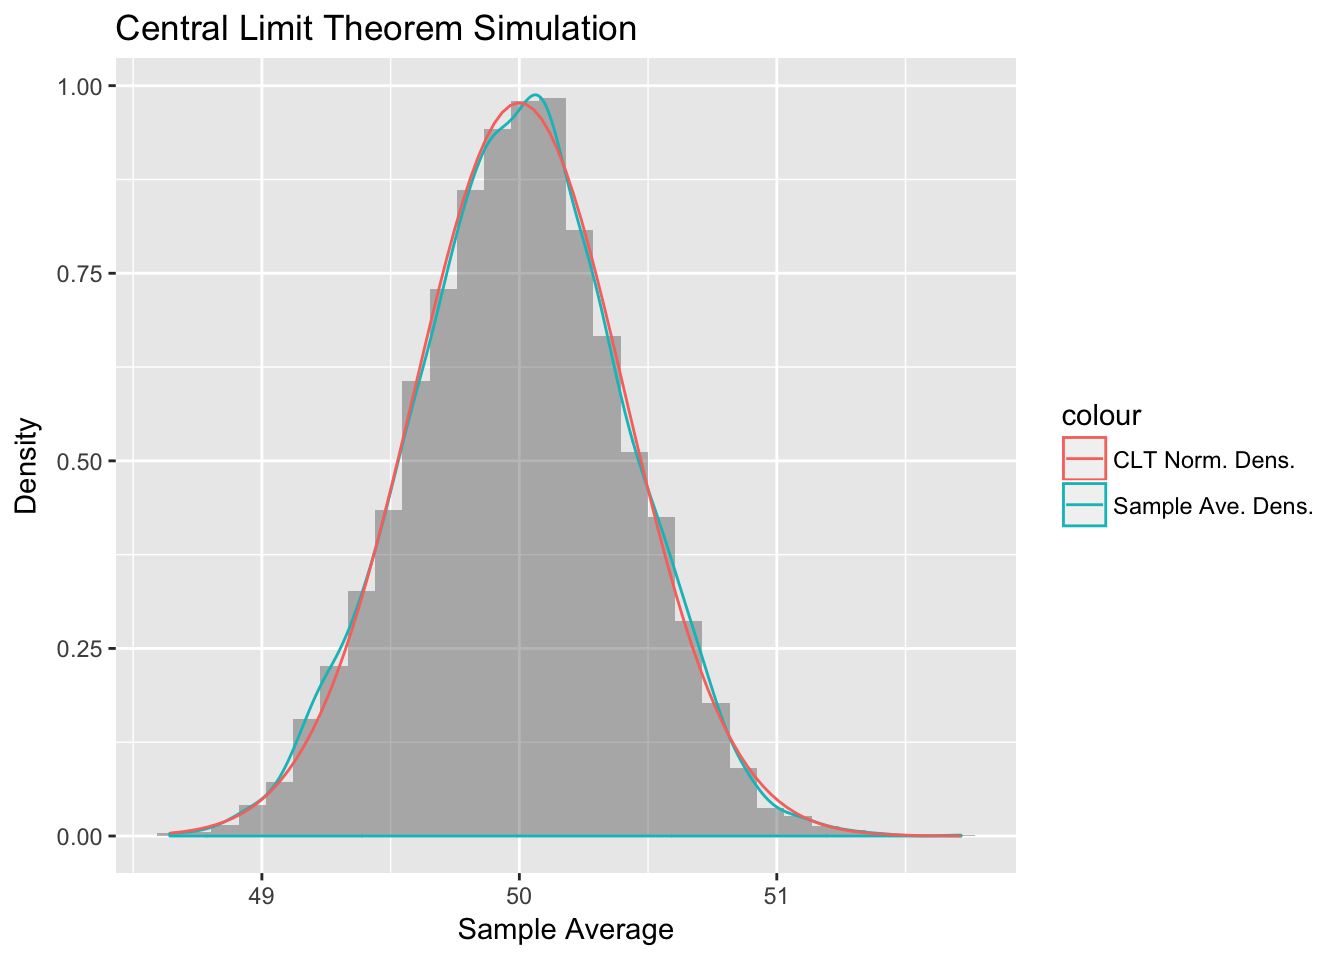
\includegraphics[height=\textheight, keepaspectratio]{cltsim}
\end{frame}


\section{Check normality}

\begin{frame}{Methods to check normality}

\begin{itemize}
  \item Explorative data analysis (EDA)
  \begin{itemize}
    \item Histogram
    \item Density plot
    \item Quantile-Quantile plot
  \end{itemize}
  \item Statistical tests
  \begin{itemize}
    \item Shapiro-Wilk normality test
    \item Anderson-Darling normality test
  \end{itemize}
\end{itemize}

\end{frame}

\subsection{Use EDA to check normality}

\begin{frame}[fragile]{Use EDA to check normality}

Histogram: 

\begin{minted}[fontsize=\scriptsize,
               frame=lines,
               bgcolor=codegray,
               framesep=1mm]{R}
num_points <- 30
normdata2 <- rnorm(num_points)

qplot(normdata2) + 
  geom_histogram() + 
  theme_bw() + 
  ggtitle(paste("rnorm (", num_points, ")", sep=""))
\end{minted}

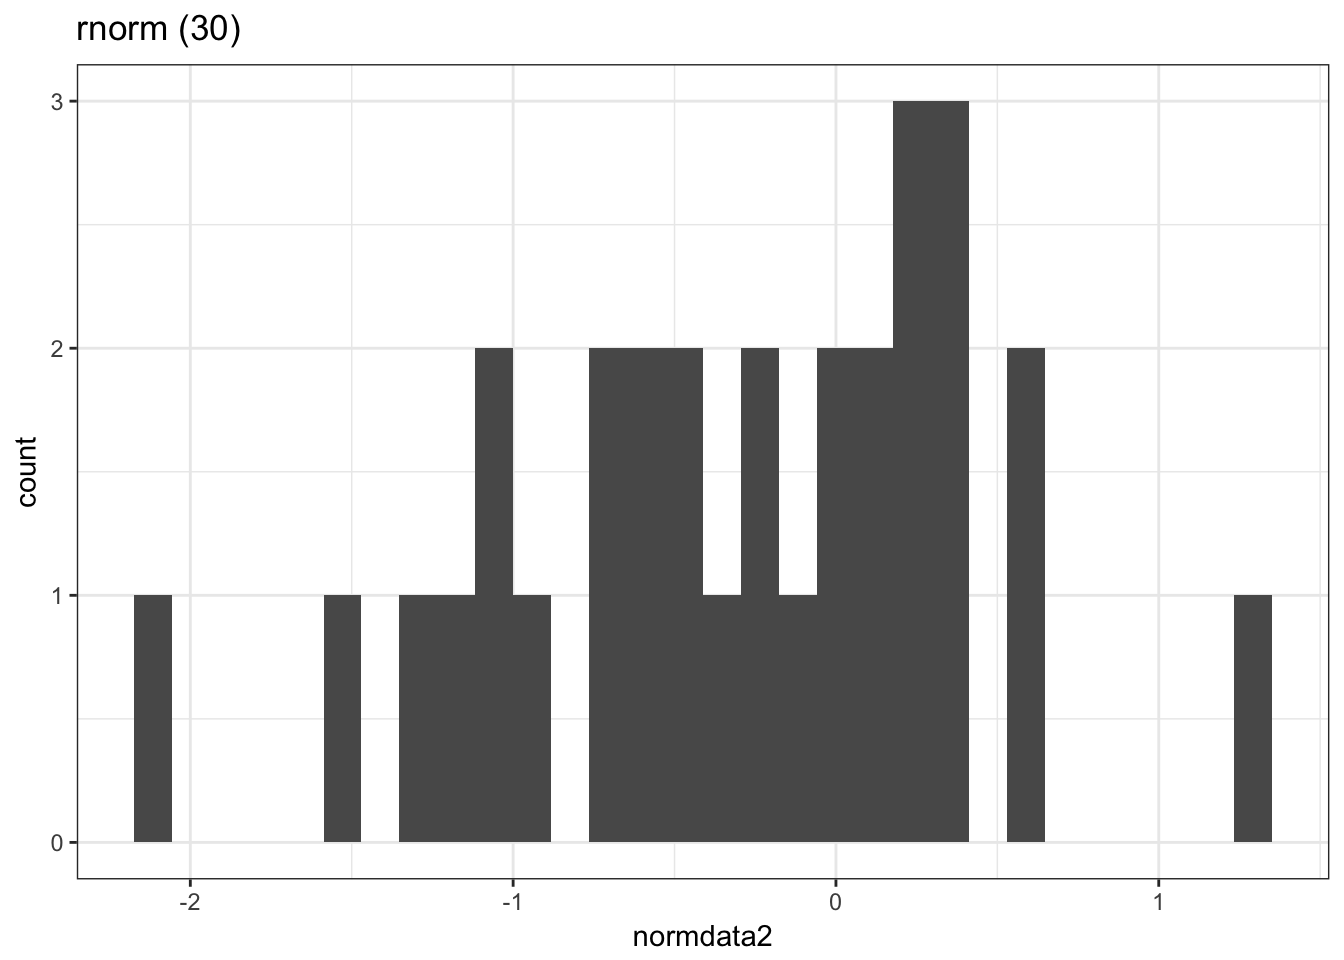
\includegraphics[height=0.4\textheight, keepaspectratio]{edahist}

\end{frame}

\begin{frame}[fragile]{Use EDA to check normality}

Quantile-Quantile (Q-Q) plot: 

\begin{minted}[fontsize=\scriptsize,
               frame=lines,
               bgcolor=codegray,
               framesep=1mm]{R}
qqnorm(normdata2, pch=16, cex=0.5, 
       main=paste("Generated using rnorm(", 
                  num_points, ")", sep=""))
qqline(normdata2, col=3)
\end{minted}
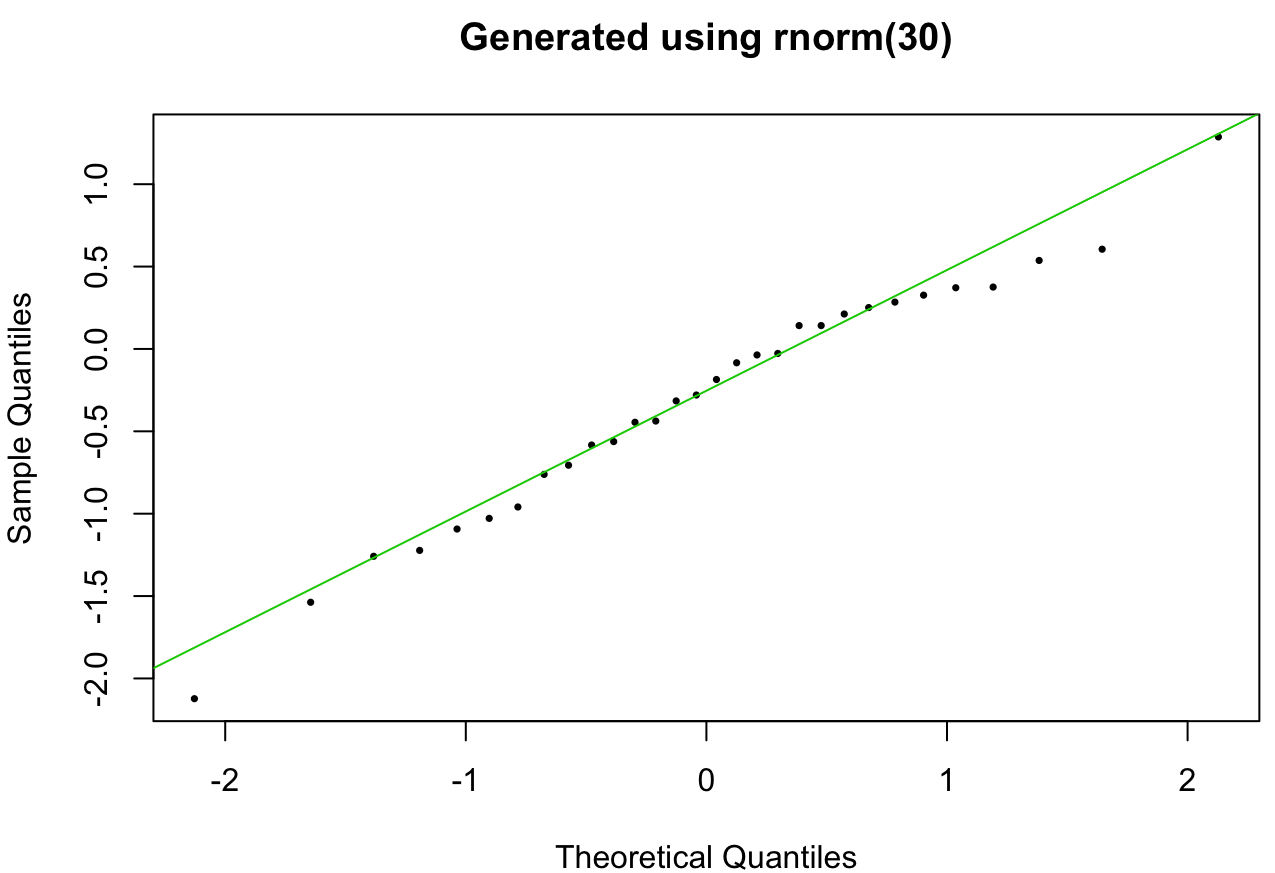
\includegraphics[height=0.6\textheight, keepaspectratio]{rnormQqPlot}

\end{frame}

\begin{frame}[fragile]{Q-Q plot}
\alert{Quantiles} divide probility distribution or sample observations into even intervals. 

Example, 4-quantiles (quartiles) and 100-quantiles (percentiles): 

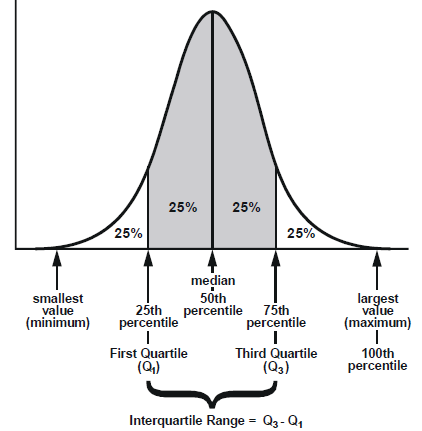
\includegraphics[height=0.6\textheight, keepaspectratio]{quantile}

\source{\url{http://my.ilstu.edu/~gjin/hsc204-hed/Module-5-Summary-Measure-2/Module-5-Summary-Measure-26.html}}

\end{frame}


\begin{frame}[fragile]{Q-Q plot}
\alert{Q-Q plot} compares the quantiles of one sample or distribution against the other. 
\vspace{-3mm}

\begin{minted}[fontsize=\scriptsize,
               frame=lines,
               bgcolor=codegray]{R}
quantile(0:10, probs=seq(0, 1, 0.1))
##   0%  10%  20%  30%  40%  50%  60%  70%  80%  90% 100% 
##    0    1    2    3    4    5    6    7    8    9   10
qqnorm(0:10, ylim = c(0,10))
qqline(0:10, ylim = c(0,10))
\end{minted}

\vspace{-5mm}
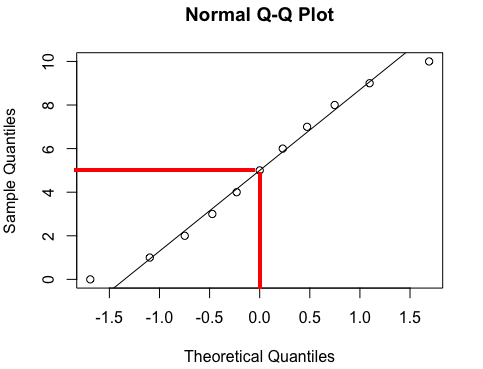
\includegraphics[height=0.5\textheight, keepaspectratio]{seq0to10qq}

\end{frame}

\begin{frame}[fragile]{Histogram of TCGA-LUAD cigarettes per day}
\begin{minted}[fontsize=\scriptsize,
               frame=lines,
               bgcolor=codegray]{R}
luad_cpd_sd <- sd(tcga_luad$cigarettes_per_day, 
                  na.rm=TRUE)
luad_cpd_mean <- mean(tcga_luad$cigarettes_per_day, 
                      na.rm=TRUE)

qplot(x = cigarettes_per_day, xlim=c(-5, 10), 
      data = tcga_luad, geom = "blank") +  
  geom_histogram(aes(y = ..density..), 
                 alpha = 0.4) +
  geom_line(aes(y = ..density.., colour = 'Empirical'),
            stat = 'density') +  
  stat_function(fun = dnorm, 
                args = list(mean=luad_cpd_mean, 
                            sd=luad_cpd_sd), 
                aes(colour = 'Normal Approx'))  + 
  scale_colour_manual(name = 'Density', 
                      values = c('red', 'blue')) + 
  theme(legend.position = c(0.85, 0.85)) + 
  ggtitle("TCGA LUAD: Cigarettes Per Day")
\end{minted}
\end{frame}

\begin{frame}{Histogram of TCGA-LUAD cigarettes per day}
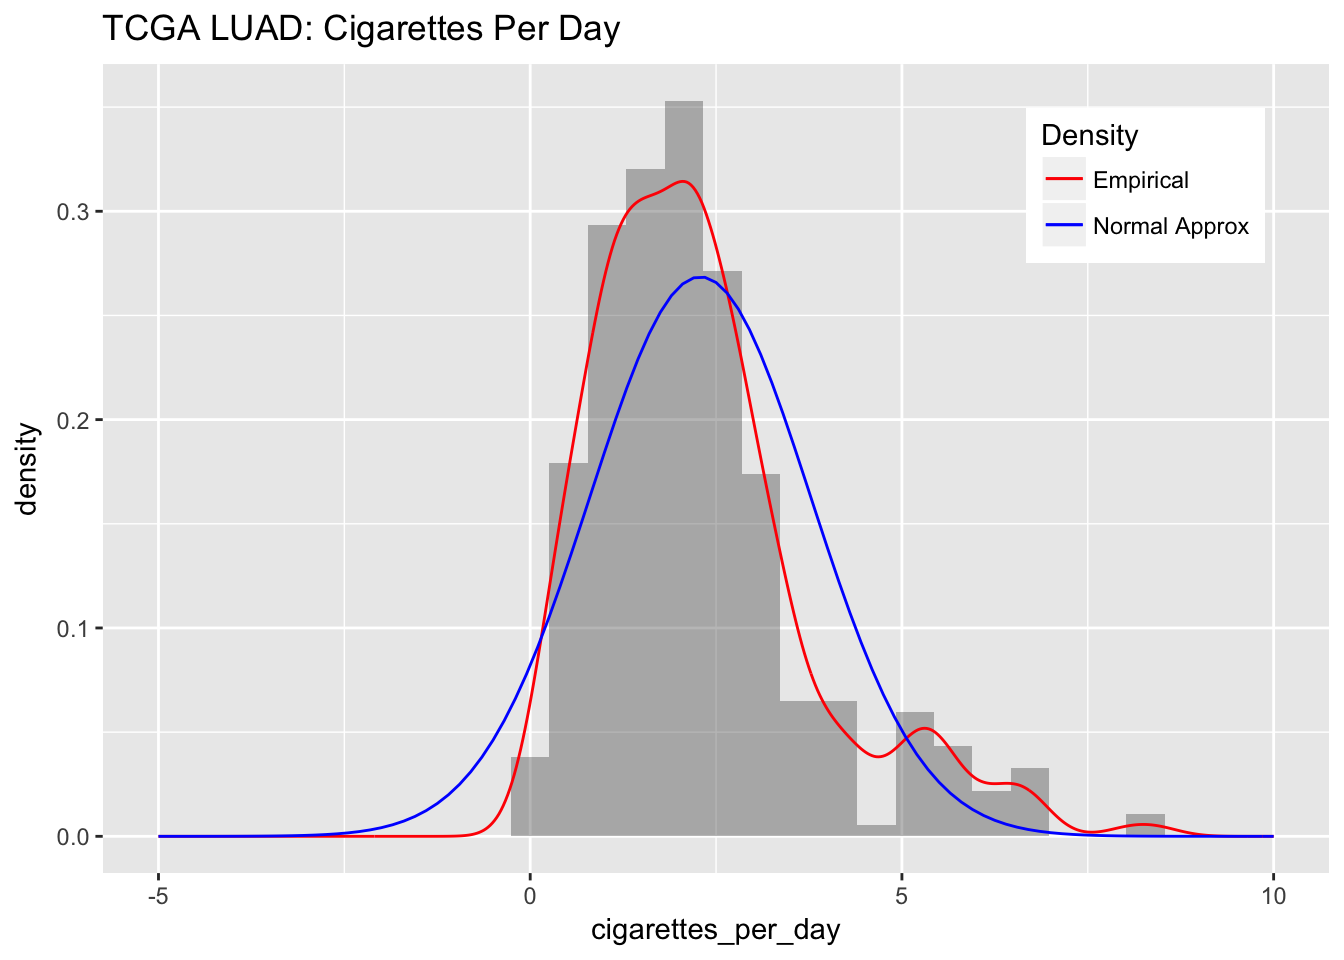
\includegraphics[width=\textwidth, keepaspectratio]{histCpd}
\end{frame}


\begin{frame}[fragile]{Q-Q plot of TCGA-LUAD cigarettes per day}
\begin{minted}[fontsize=\scriptsize,
               frame=lines,
               bgcolor=codegray]{R}
qqnorm(tcga_luad$cigarettes_per_day, 
       pch=16, cex=0.5, main="TCGA-LUAD: Cigarettes per Day")
qqline(tcga_luad$cigarettes_per_day, col=3)
\end{minted}
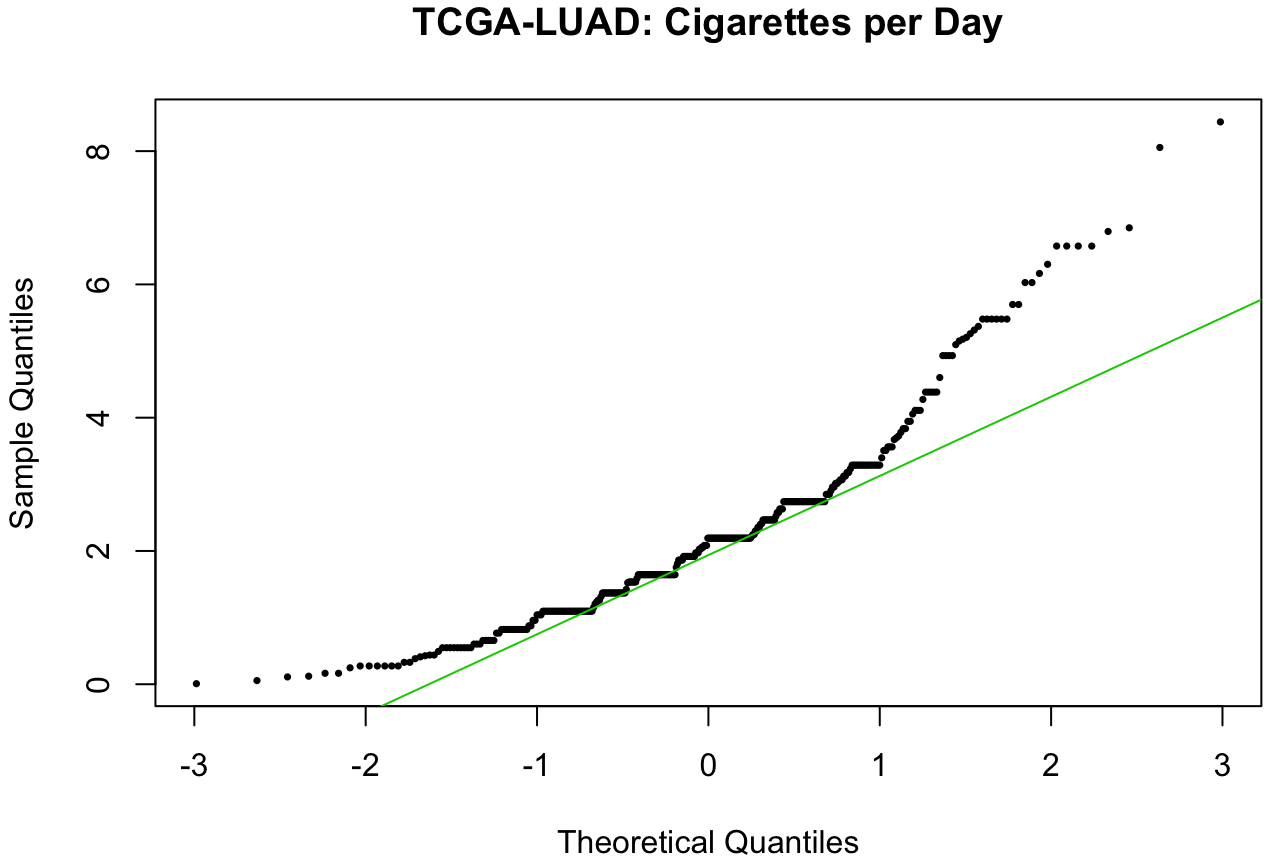
\includegraphics[height=0.6\textheight, keepaspectratio]{qqCpd}
\end{frame}


\begin{frame}{Histogram of TCGA-LUAD years smoked}
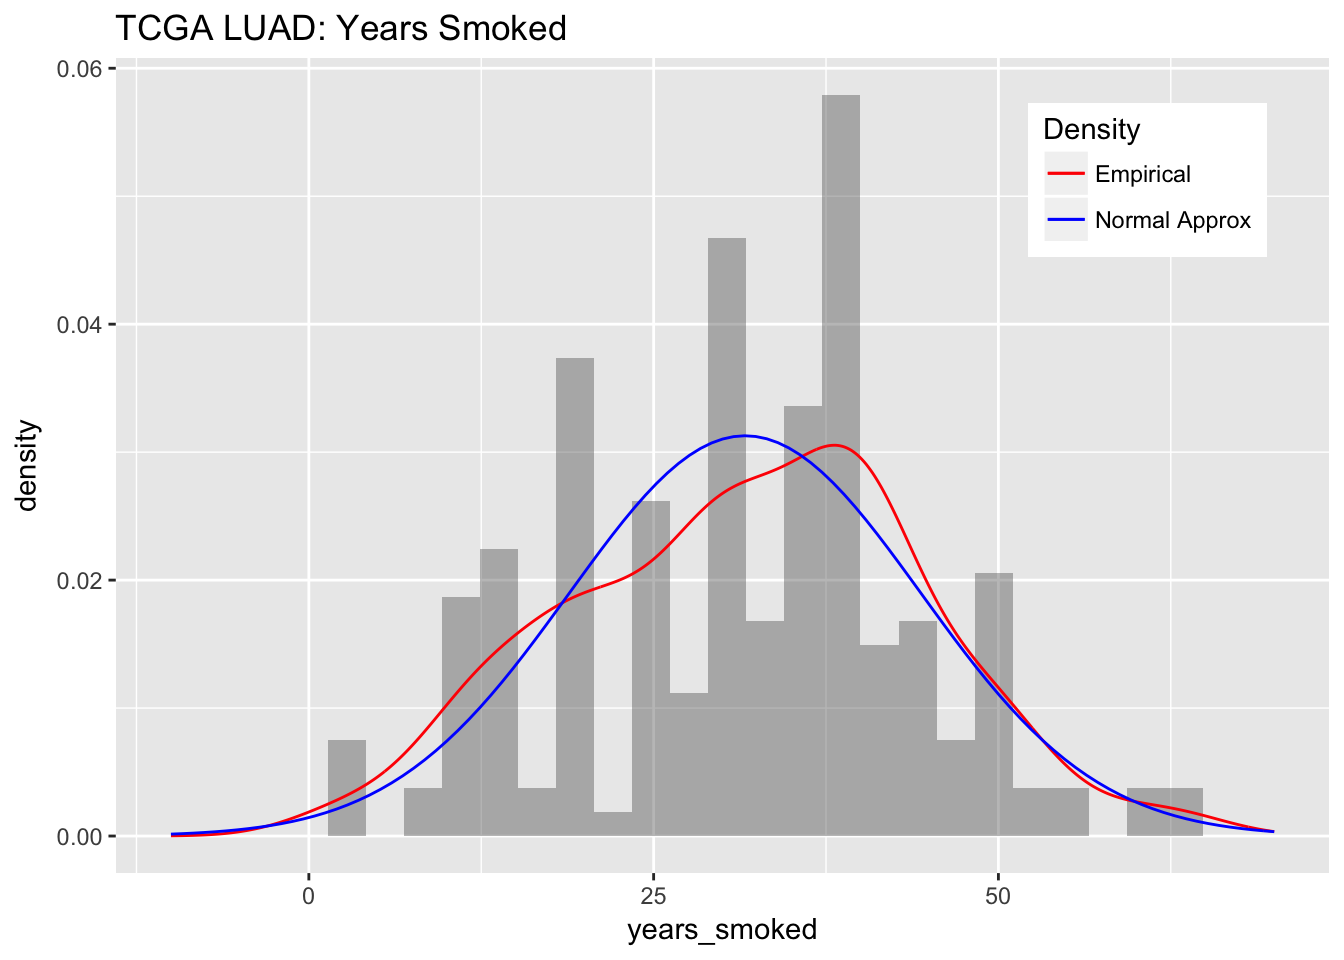
\includegraphics[width=\textwidth, keepaspectratio]{histys}
\end{frame}

\begin{frame}{Q-Q plot of TCGA-LUAD years smoked}
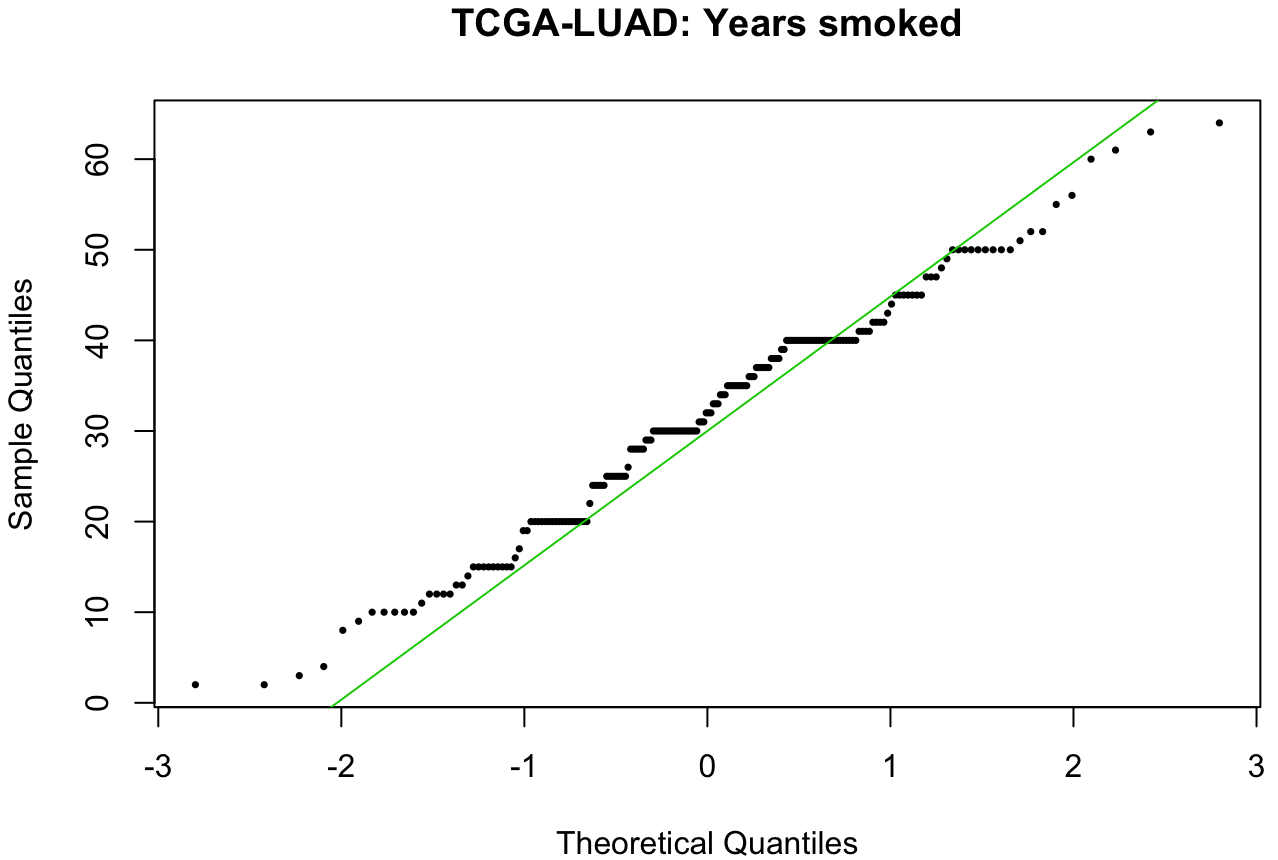
\includegraphics[width=\textwidth, keepaspectratio]{qqys}
\end{frame}

\subsection{Use statistical tests to check normality}

\begin{frame}[fragile]{Use statistical tests to check normality}
Shapiro-Wilk normality test:
\begin{minted}[fontsize=\scriptsize,
               frame=lines,
               bgcolor=codegray]{R}
nortest_points <- 100
normdata_nortest <- rnorm(nortest_points)
shapiro.test(normdata_nortest)
## 
##  Shapiro-Wilk normality test
## 
## data:  normdata_nortest
## W = 0.97583, p-value = 0.06271
shapiro.test(1:1000)
## 
##  Shapiro-Wilk normality test
## 
## data:  1:1000
## W = 0.95481, p-value < 2.2e-16

# Smaller p-value indicates significant deviation from normal 
# distribution. 
\end{minted}


\end{frame}

\begin{frame}[fragile]{Use statistical tests to check normality}
Anderson-Darling normality test

\begin{minted}[fontsize=\scriptsize,
               frame=lines,
               bgcolor=codegray]{R}
ad.test(normdata_nortest)
## 
##  Anderson-Darling normality test
## 
## data:  normdata_nortest
## A = 0.38284, p-value = 0.3912
ad.test(1:1000)
## 
##  Anderson-Darling normality test
## 
## data:  1:1000
## A = 11.085, p-value < 2.2e-16

# Smaller p-value indicates significant deviation from normal 
# distribution. 
\end{minted}

\end{frame}


\begin{frame}[fragile]{Shapiro-Wilk test of TCGA-LUAD cigarettes per day}
\begin{minted}[fontsize=\scriptsize,
               frame=lines,
               bgcolor=codegray]{R}
shapiro.test(tcga_luad$cigarettes_per_day)
## 
##  Shapiro-Wilk normality test
## 
## data:  tcga_luad$cigarettes_per_day
## W = 0.90998, p-value = 9.873e-14
\end{minted}
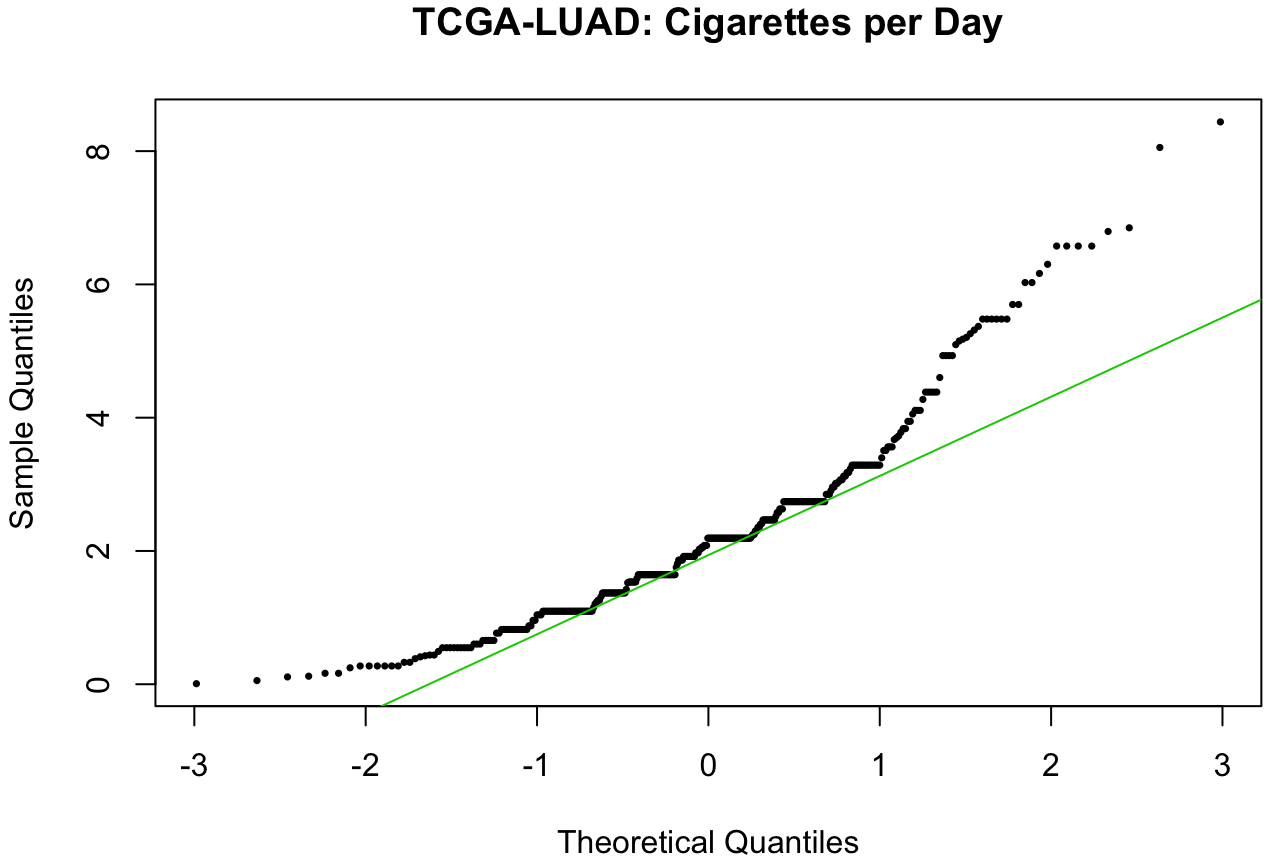
\includegraphics[height=0.6\textheight, keepaspectratio]{qqCpd}
\end{frame}


\begin{frame}[fragile]{Shapiro-Wilk test of TCGA-LUAD years smoked}
\begin{minted}[fontsize=\scriptsize,
               frame=lines,
               bgcolor=codegray]{R}
shapiro.test(tcga_luad$years_smoked)
## 
##  Shapiro-Wilk normality test
## 
## data:  tcga_luad$years_smoked
## W = 0.98572, p-value = 0.04686
\end{minted}
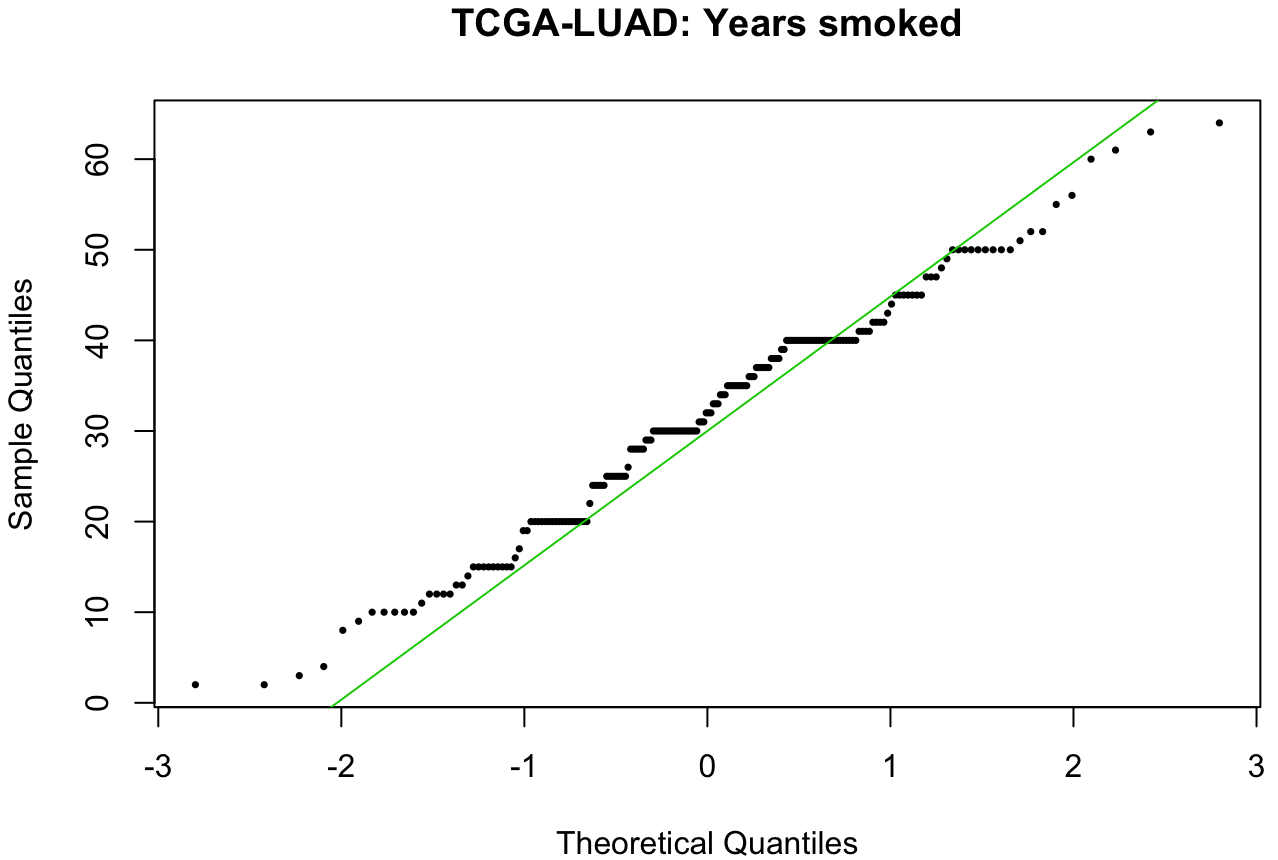
\includegraphics[height=0.6\textheight, keepaspectratio]{qqys}
\end{frame}



\section{One-sample tests of proportion}

\begin{frame}{One-sample tests of proportion}
\begin{itemize}
  \item z-test
  \item $\chi^2$-test using \code{prop.test}
  \item One-sided
  \item Two-sided
  \item Power analysis
  
\end{itemize}

\end{frame}

\begin{frame}{Overview of one-sample tests of proportion}
\begin{itemize}
  \item Proportion: $$\frac{\text{The number of observations with certain condition}}{\text{The number of total observations}}$$
  \item Qusetion: How likely the observed proportion ($prop_{obs}$) is different from another proportion ($prop_{H_0}$)?
  \begin{itemize}
    \item $prop_{obs}$ is determined by observations.
    \item $prop_{H_0}$ is determined by us when specifying the null hypothesis ($H_0$).
  \end{itemize}
  
\end{itemize}
\end{frame}


\subsection{z-test}

\begin{frame}[fragile]{z-test}

$$z = \frac{\hat{p} -p_0}{\sqrt{\frac{p_0 (1- p_0)}{n}}}$$

Intuition: apply central limit theorem on $n$ random variales $i.i.d.$ Bernoulli distribution.
\end{frame}

\begin{frame}[fragile]{z-test}

Example: A new study is performed where 22 out of 200 patients smoked more than 5 cigarettes per day. We would like to check if this group of patients has a statistically greater proportion of heavy smokers compared to the TCGA study. In TCGA, the porportion of heavy smokers 0.1. 

Null hypothesis: The porportion of heavy smokers in this new study is no more than the porportion of heavy smokers in the TCGA study. 

\end{frame}

\begin{frame}[fragile]{z-test}
Null hypothesis: The porportion of heavy smokers in this new study is no more than 0.1. 

\begin{minted}[fontsize=\scriptsize,
               frame=lines,
               bgcolor=codegray]{R}
alpha <- 0.05
z0 <- qnorm(1 - alpha)
print(z0)
## [1] 1.644854

prop2 <- 22/200
p0 <- 0.1
n <- 200

z <- (prop2 - p0)/sqrt(p0 * (1 - p0)/n)
print(z)
## [1] 0.4714045

z >= z0
## [1] FALSE
\end{minted}
\end{frame}

\subsection{\texorpdfstring{$\chi^2$}{chi-squared}-test}

\begin{frame}[fragile]{$\chi^2$-test}
Intuition: z-test with multiple catogries. For each category, apply central limit theorem on $n$ random variales $i.i.d.$ Bernoulli distribution.

$$X^2 = \sum_{i=1}^{k}\frac{(x_i - n p_i)^2}{n p_i}$$

There are $k$ total categories and $n$ total observations. $x_i$ is the number of observations of category $i$. $p_i$ is the hypothesized probability of observing category $i$. 

$X^{2}$ followed the $\chi^{2}$ distribution with $(k-1)$ degrees of freedom.
 

\end{frame}

\begin{frame}[fragile]{$\chi^2$-test}

Null hypothesis: The porportion of heavy smokers in the new study is no more than 0.1. 

\begin{Rcode}
alpha = 0.05
z0 = qnorm(1 - alpha)
print(z0)
## [1] 1.644854
hs = 22
p0 = 0.1
n2 = 200

propresult <- prop.test(hs, n2, p = p0, correct = FALSE, 
                        alternative = "greater")
\end{Rcode}
\end{frame}

\begin{frame}[fragile]{$\chi^2$-test}

\begin{Rcode}
print(propresult)
## 
##  1-sample proportions test without continuity correction
## 
## data:  hs out of n2, null probability p0
## X-squared = 0.22222, df = 1, p-value = 0.3187
## alternative hypothesis: true p is greater than 0.1
## 95 percent confidence interval:
##  0.0786844 1.0000000
## sample estimates:
##    p 
## 0.11
\end{Rcode}
\end{frame}

\begin{frame}[fragile]{$\chi^2$-test}

\begin{minted}[fontsize=\scriptsize,
               frame=lines,
               bgcolor=codegray,
               framesep=1mm]{R}
# Comparing prop.test to z-score method.
Xstat <- propresult$statistic[[1]]
print(sqrt(Xstat))
## [1] 0.4714045

z = (hs/n2 - p0)/sqrt(p0 * (1 - p0)/n2)
print(abs(z))
## [1] 0.4714045
\end{minted}

\end{frame}


\subsection{One-sided versus two-sided test}

\begin{frame}{One-sided versus two-sided test}
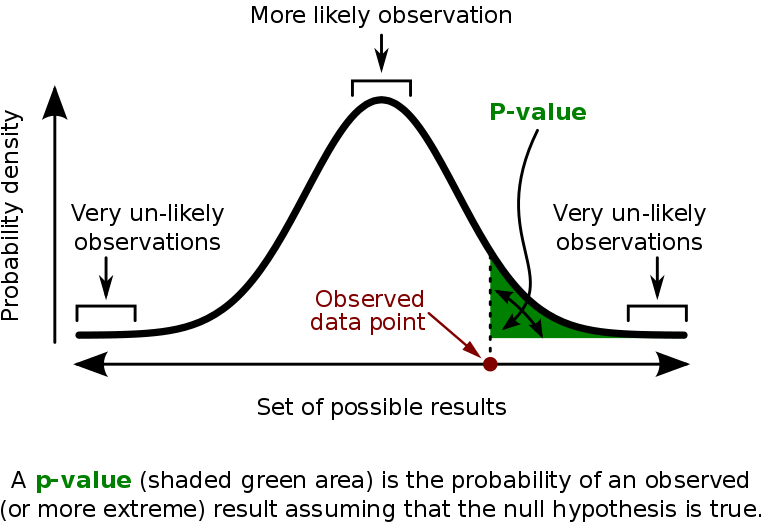
\includegraphics[width=\textwidth, keepaspectratio]{pval}
\source{\url{https://en.wikipedia.org/wiki/One-_and_two-tailed_tests}}
\end{frame}

\begin{frame}{One-sided versus two-sided test}
One-sided:

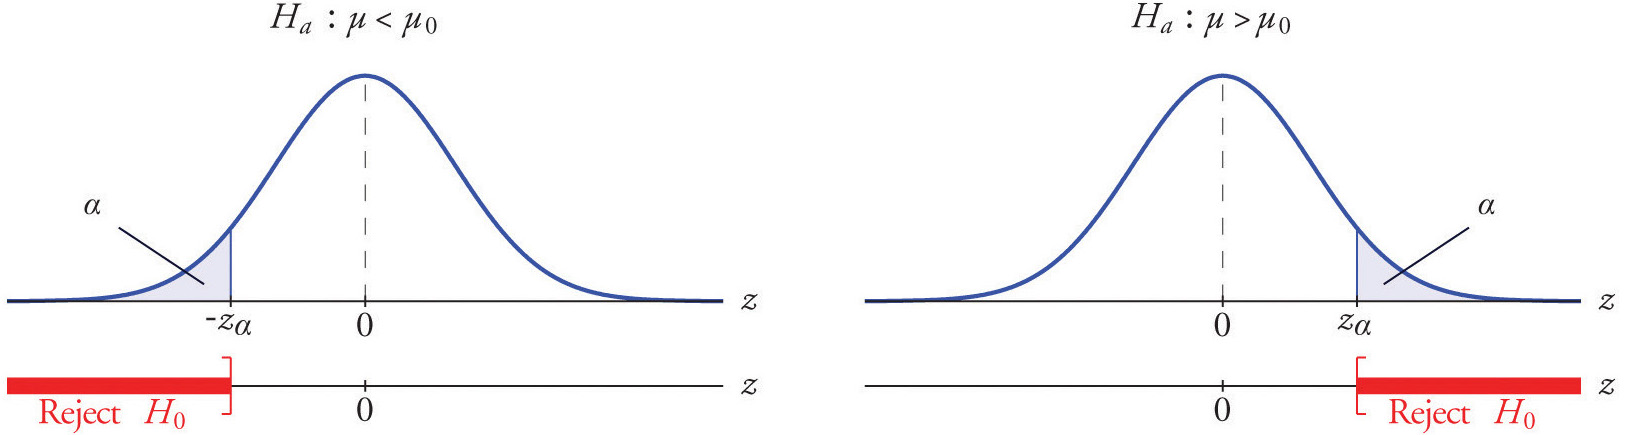
\includegraphics[height=0.3\textheight, keepaspectratio]{1sided}

Two-sided:

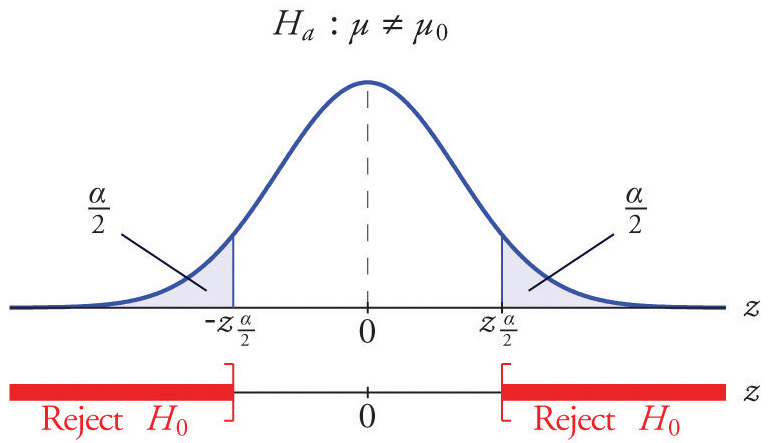
\includegraphics[height=0.3\textheight, keepaspectratio]{2sided}

\source{\href{https://catalog.flatworldknowledge.com/bookhub/reader/3318?e=fwk-shafer-ch08_s02}{flatworldknowledge}}
\end{frame}



\begin{frame}[fragile]{Two-sided one sample test of proportion}

\begin{Rcode}
hs = 30  # second study patient proportion 
p0 = 0.1  # TCGA LUAD proportion
n2 = 200  # second study sample size
z_twotail = (hs/n2 - p0)/sqrt(p0 * (1 - p0)/n)
pval_z_twotail = 2 * pnorm(z_twotail, lower.tail = FALSE)
pval_z_twotail
## [1] 0.01842213

proptest_twotail <- prop.test(hs, n2, p = p0, correct = FALSE, 
                              alternative = "two.sided")
proptest_twotail$p.value
## [1] 0.01842213
\end{Rcode}

\tikzoverlay[text height=30mm] at (50mm, 20mm) {
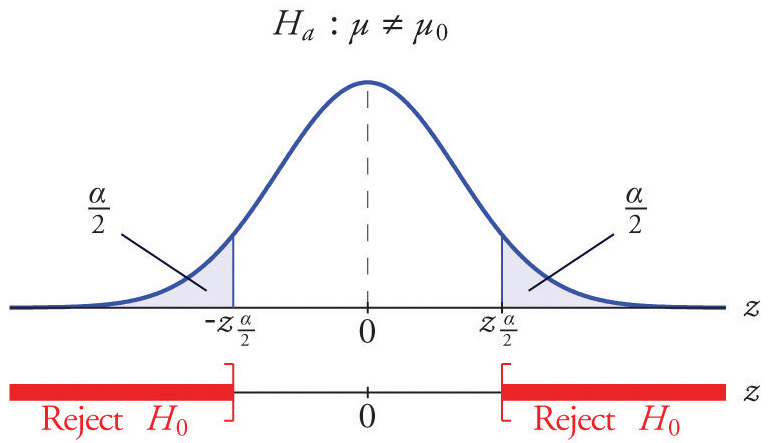
\includegraphics[height=30mm, keepaspectratio]{2sided}
};
\end{frame}

\begin{frame}[fragile]{One-sided one sample test of proportion}

\begin{Rcode}
hs = 22  # second study heavy smokers
p0 = 0.1  # TCGA LUAD proportion
n2 = 200  #Number of tests

propresult <- prop.test(hs, n2, p = p0, correct = FALSE, 
                        alternative = "greater")
propresult$p.value
## [1] 0.3186759

z = (hs/n2 - p0)/sqrt(p0 * (1 - p0)/n2)
print(abs(z))
## [1] 0.4714045
pvalue_z_onesided <- pnorm(-abs(z))
pvalue_z_onesided
## [1] 0.3186759
\end{Rcode}

\tikzoverlay[text width=45mm] at (65mm, 30mm) {
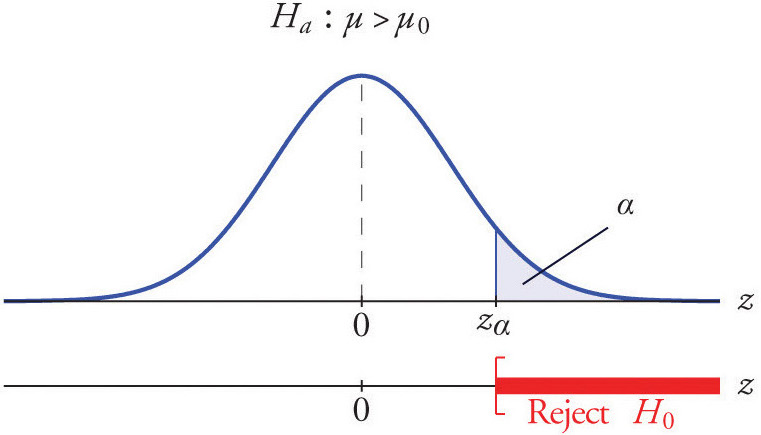
\includegraphics[width=45mm, keepaspectratio]{altg}
};

\end{frame}

\subsection{Power analysis}

\begin{frame}{Power analysis for one-sample test of proportion}
\begin{itemize}
  \item The \alert{power} of a binary hypothesis test is the probability that the test correctly rejects the null hypothesis ($H_0$) when a specific alternative hypothesis ($H_1$) is true. $$\text{power} = \Pr {\big (}{\text{reject }}H_{0}\mid H_{1}{\text{ is true}}{\big )}$$
  \item Main factors in calculating the power of a test:
  \begin{itemize}
    \item Effect size, or the difference in means between two groups
    \item Sample size: $n$
    \item Significance threshold, $\alpha$ (often 0.05)
  \end{itemize}
\end{itemize}

\source{\url{https://en.wikipedia.org/wiki/Statistical_power}}
\end{frame}

\begin{frame}[fragile]{Power analysis for one-sample test of proportion}

Calculate power given effect size, sample size, and significance threshold.

\begin{Rcode}
# h is effect size
pwr.p.test(h = 0.5, n = 55, sig.level = 0.05)
## 
##      proportion power calculation for binomial distribution 
##      (arcsine transformation) 
## 
##               h = 0.5
##               n = 55
##       sig.level = 0.05
##           power = 0.9597797
##     alternative = two.sided
\end{Rcode}

\end{frame}



\begin{frame}[fragile]{Power analysis for one-sample test of proportion}

Calculate sample size given power, effect size, and significance threshold.

\begin{Rcode}
pwr.p.test(h = 0.5, n = NULL, sig.level = 0.05, power = 0.9)
## 
##      proportion power calculation for binomial distribution 
##      (arcsine transformation) 
## 
##               h = 0.5
##               n = 42.02968
##       sig.level = 0.05
##           power = 0.9
##     alternative = two.sided
\end{Rcode}

\end{frame}

\begin{frame}[fragile]{Power analysis for one-sample test of proportion}

Calculate effect size given power, sample size, and significance threshold.

\begin{Rcode}
pwr.p.test(h = NULL, n = 100, sig.level = 0.05, power = 0.9)
## 
##      proportion power calculation for binomial distribution 
##      (arcsine transformation) 
## 
##               h = 0.3241514
##               n = 100
##       sig.level = 0.05
##           power = 0.9
##     alternative = two.sided
\end{Rcode}

\end{frame}

\begin{frame}[fragile]{Power analysis for one-sample test of proportion}

Estimate effect size \code{h} using \code{ES.h}. 

\begin{Rcode}
pwr.p.test(h = ES.h(p1 = 0.75, p2 = 0.5), sig.level = 0.05, 
           n = NULL, power = 0.8, 
           alternative = "greater")
## 
##      proportion power calculation for binomial distribution 
##      (arcsine transformation) 
## 
##               h = 0.5235988
##               n = 22.55126
##       sig.level = 0.05
##           power = 0.8
##     alternative = greater
\end{Rcode}

\end{frame}

\begin{frame}[c]
  \large{Questions?}
\end{frame}


% \appendix
% \section{Appendix}
% 
% \begin{frame}[fragile]{Backup slides}
%   Test
% \end{frame}
% 
% \begin{frame}[allowframebreaks]{References}
% 
% %  \bibliography{demo}
% %  \bibliographystyle{abbrv}
% 
% \end{frame}
% 
% \begin{frame}{Test}
% 
% %  \bibliography{demo}
% %  \bibliographystyle{abbrv}
% 
% \end{frame}

\end{document}
